\chapter{Samplers: Framework Android}




\section{Jerarquía de Clases}
Nuestras clases, las que permiten que se cree una app

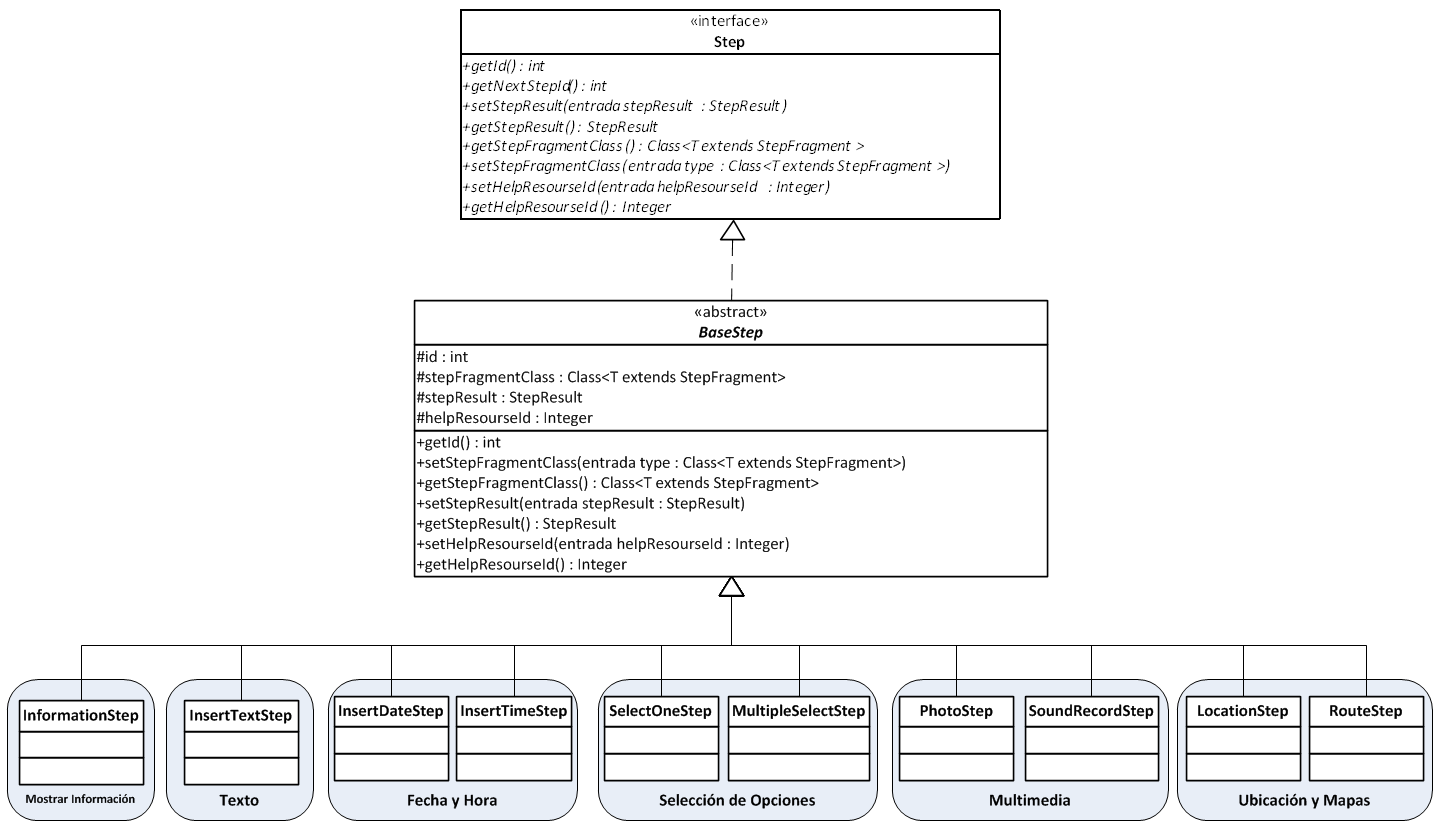
\includegraphics[scale=0.4]{05-implementacion/Steps.png} 


\subsection{Workflow: Control de Ejecución}

\subsubsection{Step, el Paso}

\subsubsection{StepResult, El Resultado de la Ejecución del Paso}

\subsubsection{Muestra, Conjunto de Resultados}

\subsection{Envío de Muestras a Servidor Web}
Acá explicamos un poco la estrategia que utilizamos para el envío de muestras y las librerías externas que nos ayudaron.

\section{Instalación y uso del framework}
\subsection{Instalación}
Instalación. 
Requerimientos mínimos:
\begin{itemize}
\item Android Studio (Java): Si bien esta pensado para y probado en Android Studio, podria funcionar bien en otro entorno que use Java y deje importar archivos Android Archive (.aar).
\item Android SDK API17: Android 4.2 (Jelly Bean) o superior.
\end{itemize}

Instalación:
\begin{enumerate}
	\item Crear en Android Studio un nuevo proyecto vacío (sin ninguna Activity).
		\begin{itemize}
		\item Seleccionar API17 o superior como versión mínima de Android SDK
		\end{itemize}
	\item Importar la librería del framework en el proyecto creado
		\begin{itemize}
		\item Descargar la última versión de samplersFramework.aar desde https://github.com/			cientopolis/samplers/releases/
		\item Importar la librería al proyecto: File -> New -> New Module -> Import .JAR/.AAR Package
		\end{itemize}
	\item Agregar el repositorio de Google
		\begin{itemize}
			\item En el archivo build.gradle del proyecto agregar: 
			\begin{lstlisting}[language=XML, frame=single]
allprojects {
    repositories {
        jcenter()
        google()
    }
}
			\end{lstlisting}	
		\end{itemize}
	\item Agregar las dependencias necesarias:
		\begin{itemize}
			\item En el archivo build.gradle de la aplicación agregar: 
			\begin{lstlisting}[language=XML, frame=tlb]
dependencies {
  // here the standards dependencies created by Android Studio
  // ...

  // if not added automatically, add this dependency 
  // you should use the latest version e.j. 25.+
  compile 'com.android.support:design:24.2.1' 
  compile 'com.android.support.constraint:constraint-layout:1.0.2'

  // if you will use maps and location services, add this dependencies (you should use the latest version)
  compile ('com.google.android.gms:play-services-location:12.0.1')
  compile ('com.google.android.gms:play-services-maps:12.0.1')
  
  // if you will use authentication with Google, add this dependencies (you should use the latest version)
  compile ('com.google.android.gms:play-services-auth:12.0.1')

  // the framework dependency
  compile project(":samplersFramework")
}
			\end{lstlisting}	
		\end{itemize}	

	\item Instanciar:
		\begin{itemize}
		\item La instanciación puede ser manual o usando el generador de clases en Gradle como se explica en la siguiente sección.
		\end{itemize}
\end{enumerate}	

\subsection{Instanciación}
Una vez instalado el framework...
La instanciación puede ser manual o usando el generador de clases de Gradle.

\subsubsection{Instanciación manual}
Básicamente se tiene que crear un objeto Workflow, agregarle los objetos Steps, y llamar a la activity TakeSampleActivity pasándole el workflow como parámetro.
También es necesario establecer la configuración general en el método onCreate de la activity principal (main activity).
Se puede usar una activity principal propia o se puede heredar de SamplersMainActivity. En ambos casos se debe hacer lo siguiente:
\begin{itemize}
	\item Establecer la configuración general en el método onCreate de la activity principal:
		\begin{lstlisting}[language=Java, frame=tlb]
NetworkConfiguration.setURL("http://192.168.1.10/samplers/upload.php");
NetworkConfiguration.setPARAM_NAME_SAMPLE("sample");
// Optional if you will use authentication
NetworkConfiguration.setPARAM_NAME_USER_ID("user_id");
NetworkConfiguration.setPARAM_NAME_AUTHENTICATION_TYPE("authentication_type");

// Optional if you will use authentication, set the configuration
AuthenticationManager.setAuthenticationEnabled(true);
AuthenticationManager.setAuthenticationOptional(true);
		\end{lstlisting}

	\item Crear un Workflow. Si se está heredando de SamplersMainActivity se debe hacer sobreescribiendo el método onCreate.
		\begin{lstlisting}[language=Java, frame=tlb]
@Override
protected Workflow getWorkflow() {
	Workflow workflow = new Workflow();
    	
	Step step = new InformationStep(2,"Por favor tome una foto de su gato", null);
	workflow.add(step);
    	
	step = new PhotoStep(1,"Bienvenido a la app de prueba", 2);
	workflow.add(step);
    	
	return workflow;
    	
}		
		\end{lstlisting}
Nota: en el ejemplo anterior se muestra un Workflow que tiene dos Steps. El primero muestra un mensaje de bienvenida y el segundo pide para tomar una foto. Para ver los distintos Steps que se pueden usar vea la sección de Steps.

	\item Iniciar la activity TakeSampleActivity. Si se está heredando de SamplersMainActivity esto se hace solo en el método onClick del botón "tomar muestra". De lo contrario, deberá iniciarla de la siguiente forma, en el método onClick de un botón por ejemplo:
		\begin{lstlisting}[language=Java, frame=tlb]
@Override
public void takeSampleClick(View view) {
	Workflow workflow = getWorkflow();

	Intent intent = new Intent(this, TakeSampleActivity.class);        
	intent.putExtra(TakeSampleActivity.EXTRA_WORKFLOW, workflow);
	startActivity(intent);
    	
}		
		\end{lstlisting}




\end{itemize}


\subsubsection{Instanciación usando el  generador de clases de Gradle}

Básicamente, el generador de clases de Gradle se encarga de hacer una instanciación manual a partir de un archivo de configuración (JSON). Está pensado para desarrolladores que no tienen muchos conocimientos en Android, o para servir de interfaz entre una aplicación que genere apps a través de Samplers (esto hay que escribirlo mejor).

Los pasos para usar el generador de clases de Gradle son:
\begin{enumerate}
	\item Crear un archivo JSON con el nombre SamplersConfig.json
		\begin{itemize}
			\item El formato y las opciones están explicadas en la siguiente sección.
			\item Para validar sintaxis se puede usar el validador online: jsonformatter.curiousconcept.com (Ver si se puede poner esto o hay que tener permisos?)
			\item Al final de la sección se provee un archivo de ejemplo
		\end{itemize}
		
	\item Copiar el archivo creado en el item anterior al directorio raíz del proyecto Android
	
	\item Descargar la última versión de los archivos \textbf{samplers.gradle} y \textbf{samplersclassgenerator.jar} del repositorio de Samplers (https://github.com/cientopolis/samplers/releases/) y copiarlos también al directorio raíz del proyecto Android
	
	\item Enlazar el archivo samplers.gradle en el archivo build.gradle de la aplicación
		\begin{itemize}
			\item Android Studio crea por defecto dos archivos build.gradle, uno a nivel de aplicación y otro a nivel de proyecto. Debe usarse el de aplicación
			\item Al final del archivo build.gradle de aplicación agregar:
\begin{lstlisting}[language=XML, frame=tlb]
apply from: '../samplers.gradle'
\end{lstlisting}
			\item Al guardar los cambios, Android Studio sugerirá hacer una sincronización del proyecto, hacerla. Esto generará en la aplicación una activity llamada MyMainSamplersActivity en base a las opciones configuradas en el archivo SamplersConfig.json.
			\item Si se necesita volver a generar esta activity (si se quieren modificar algunas opciones por ejemplo ) se puede eliminar la misma, hacer las modificaciones en el archivo SamplersConfig.json y volver a generar el proyecto (en el menu Build -> Make Project)
		\end{itemize}
		
	\item Eliminar o (customizar) el archivo \textbf{style.xml} que está en \textbf{res/values} en la aplicación
	
	\item Ejecutar la aplicación y listo.

\end{enumerate}


\subsection{Secciones del Archivo}

El archivo SamplersConfig.json es un archivo JSON con 3 objetos:
\begin{itemize}
	\item El objeto \textbf{project}
		
	El objeto project tiene dos campos
	\begin{itemize}
		\item \textbf{app\_path}: Un String con la ubicación del directorio de los fuentes de la aplicación, relativo al directorio del proyecto. Es donde están los archivos -java de la aplicación y donde se creará el archivo MyMainSamplersActivity.java
		\item \textbf{package\_name}: Un String con el nombre del package usado para las activities de la aplicación. Es el package donde la activity MyMainSamplersActivity será agregada.
	\end{itemize}
	
Ejemplo:
\begin{lstlisting}[language=XML, frame=tlb]	
{
  "project" : {
    "app_path" = "app/src/main/java/com/example/myApplication/"
    "package_name" : "com.example.myApplication"
  }
}
\end{lstlisting}	
	
	\item El objeto \textbf{application}
	El objeto application tiene 7 campos, de los cuales 3 son requeridos y los otros 4 opcionales (para habilitar características especiales)
	\begin{itemize}
		\item \textbf{title}: Un String con el nombre de la aplicación.
		
		 \item \textbf{welcomeMessage}: Un String con el mensaje de bienvenida que se mostrará en la activity principal (MyMainSamplersActivity)
		 
		 \item \textbf{networkConfiguration}: Un objeto con la configuración de red que se usará para enviar las muestras al servidor web. Ver mas abajo la configuración de este objeto.
		 
		 \item \textbf{googleMaps\_API\_KEY}: [Opcional] Un String con la API Key de Google. Este campo es necesario si se van a usar los servicios de ubicación y mapas (Location Step y Route Step). La API Key de google se puede obtener desde la página de google developers (https://developers.google.com/maps/documentation/android-api/signup)
		 
		 \item \textbf{mainHelpFileName}: [Opcional] Un String con el nombre del archivo HTML que contiene la ayuda principal de la aplicación. Este archivo debe estar junto con el archivo SamplersConfig.json. Ver la sección Mostrando Ayuda para mas detalles.
		 
		 \item \textbf{authenticationEnabled}: [Opcional] Un boolean que indica si se usará autenticación (true) o no (false). Si se omite este campo se asume false. Ver la sección Usando Autenticación para mas detalles.
		 
		 \item \textbf{authenticationOptional}: [Opcional] Un boolean que indica si la autenticación será opcional (true) o requerida (false). Si se omite este campo se asume true (autenticación opcional). Este campo solo tiene sentido si se usa autenticación. Ver la sección Usando Autenticación para mas detalles.
		 
	\end{itemize}
	
	
	El objeto \textbf{networkConfiguration}:
	El objeto networkConfiguration contiene la configuración de red que se usará para enviar las muestras al servidor web. Tiene 4 campos, de los cuales 2 son requeridos y los otros 2 opcionales.
	
	\begin{itemize}
	
		\item \textbf{url}: Un String con la URL del servidor web al cual se le enviaran las muestra con un mensaje HTTP POST.
		
		\item \textbf{paramName}: Un String con el nombre del parámetro dentro del mensaje HTTP POST en el que se enviará la muestra.
	
		\item \textbf{paramNameUserId}: (Opcional) Un String con el nombre del parámetro dentro del mensaje HTTP POST en el que se enviará el id del usuario que envía la muestra. Este campo solo es necesario si se usa autenticación. Ver la sección Usando Autenticación para mas detalles.
		
		\item \textbf{paramNameAuthenticationType}: (Opcional) Un String con el nombre del parámetro dentro del mensaje HTTP POST en el que se enviará el tipo de autenticación que usó el usuario que envía la muestra. Este campo solo es necesario si se usa autenticación. Ver la sección Usando Autenticación para mas detalles.
	
	\end{itemize}
	
	
Ejemplo:
\begin{lstlisting}[language=XML, frame=tlb]
{
  "application": {
    "title" : "Samplers Hello World App",
    "welcomeMessage" : "Welcome to your first Samplers App!",
    "networkConfiguration" : {
      "url" : "http://192.168.1.10/samplers/upload.php",
      "paramName" : "sample",
      "paramNameUserId" : "user_id",
      "paramNameAuthenticationType" : "authentication_type"
    },
    "authenticationEnabled" : true,
    "authenticationOptional" : true,
    "googleMaps_API_KEY" : "your_google_maps_API_KEY",
    "mainHelpFileName" : "mainhelp.html"
  } 
}
\end{lstlisting}	
	
	
	\item El objeto \textbf{workflow}
	El objeto workflow representa el protocolo para la toma de la muestra. Son los pasos que se ejecutarán para tomar la misma.
	El objeto cuenta con dos campos:
		
	\begin{itemize}
	
		\item \textbf{actionLabel}: Un String con el título que se usará para el botón que inicia la activity TakeSampleActivity, que es la encargada de tomar la muestra.
		
		\item \textbf{steps}: Un Array de Objetos Step los cuales forman el workflow. El primer objeto del array se considera como el inicio del mismo. Ver la sección Steps para mas detalles.
	
	
	\end{itemize}	
	
	
Ejemplo:
\begin{lstlisting}[language=XML, frame=tlb]	
{
  "workflow": {
    "actionLabel" : "Tomar muestra",
    "steps": [
      {
        "id" : 1,
        "type" : "Information",
        "text" : "Por favor, siga las instrucciones",
        "nextStepId" : 2
      },
      {
        "id" : 2,
        "type" : "Location",
        "text" : "Por favor posicione la muestra en el mapa",
        "nextStepId" : 3,
        "helpFileName" : "locationhelp.html"
      },
      {
        "id" : 3,
        "type": "MultipleSelect",
        "title" : "Seleecione las cosas que ve",
        "helpFileName" : "selecthelp.html",
        "options" : [
          {
            "id":1,
            "text":"Arboles"
          },
          {
            "id":2,
            "text":"Basura"
          },
          {
            "id":3,
            "text":"Agua"
          }
        ]
      }
    ]
  }
}

\end{lstlisting}	
	
\end{itemize}

\subsection{Configuración de los Servicios de Google}

\section{Steps}
los steps son aaaaaaaaaaaaaaaaaaaaaaaaaahhhh, bueno, lo explicamos despues...

\subsection{InformationStep: Mostrar información}

En Android Studio (Java):
\begin{lstlisting}[language=Java, frame=tlb]	
InformationStep step = new InformationStep(1,"Texto para mostrar",2);
\end{lstlisting}

Usando el generador de clases:
\begin{lstlisting}[language=XML, frame=tlb]	
{
	"id":1,
	"type" : "Information",
	"text" : "Texto para mostrar",
	"nextStepId": 2
}
\end{lstlisting}

\subsubsection{InformationStepResult: El resultado de Mostrar información}

\subsection{SelectOneStep: Seleccionar una opción de un grupo de opciones}
en forma de radio buttons

En Android Studio (Java):
\begin{lstlisting}[language=Java, frame=tlb]	
ArrayList<SelectOneOption> optionsToSelectOne = new ArrayList<SelectOneOption>();
optionsToSelectOne.add(new SelectOneOption(1,"Opcion 1", 2));
optionsToSelectOne.add(new SelectOneOption(2,"Opcion 2", 2));
optionsToSelectOne.add(new SelectOneOption(3,"Opcion 3", 3));
SelectOneStep step = new SelectOneStep(1,optionsToSelectOne,"Seleccione una opcion");

\end{lstlisting}

Usando el generador de clases:
\begin{lstlisting}[language=XML, frame=tlb]	
{
  "id" : 1,
  "type" : "SelectOne",
  "title" : "Seleccione una opcion",
  "options" : [
    {
      "id":1,
      "text":"Opcion 1",
      "nextStepId" : 2
    },
    {
      "id":2,
      "text":"Opcion 2",
      "nextStepId" : 2
    },
    {
      "id":3,
      "text":"Opcion 3",
      "nextStepId" : 3
    }
  ]
}
\end{lstlisting}

\subsubsection{SelectOneStepResult: El resultado de Seleccionar una opción de un grupo de opciones}

\subsection{MultipleSelectStep: Seleccionar varias opciones de un grupo de opciones}
en forma de checkboxes

En Android Studio (Java):
\begin{lstlisting}[language=Java, frame=tlb]	
ArrayList<MultipleSelectOption> optionsToSelect = new ArrayList<MultipleSelectOption>();
optionsToSelect.add(new MultipleSelectOption(1,"Arboles"));
optionsToSelect.add(new MultipleSelectOption(2,"Basura"));
optionsToSelect.add(new MultipleSelectOption(3,"Agua"));
optionsToSelect.add(new MultipleSelectOption(4,"Animales"));
MultipleSelectStep step = new MultipleSelectStep(1,optionsToSelect,"Seleccione lo que ve",2); 
\end{lstlisting}

Usando el generador de clases:
\begin{lstlisting}[language=XML, frame=tlb]	
{
  "id" : 1,
  "type" : "MultipleSelect",
  "title" : "Seleccione lo que ve",
  "options" : [
    {
      "id":1,
      "text":"Arboles"
    },
    {
      "id":2,
      "text":"Basura"
    },
    {
      "id":3,
      "text":"Agua"
    },
    {
      "id":4,
      "text":"Animales"
    }
  ],
  "nextStepId" : 2
}
\end{lstlisting}

\subsubsection{MultipleSelectStepResult: El resultado de Seleccionar varias opciones de un grupo de opciones}

\subsection{PhotoStep: Tomar una foto}
muestra un preview
usa una camara dependiendo de la api

En Android Studio (Java):
\begin{lstlisting}[language=Java, frame=tlb]	
PhotoStep step = new PhotoStep(1,"Por favor tome una foto de su gato",2);
\end{lstlisting}

Usando el generador de clases:
\begin{lstlisting}[language=XML, frame=tlb]	
{
  "id" : 1,
  "type" : "Photo",
  "text" : "Por favor tome una foto de su gato",
  "nextStepId" : 2
}
\end{lstlisting}

\subsubsection{PhotoStepResult: El resultado de Tomar una foto}

\subsection{SoundRecordStep: Grabar sonido}

En Android Studio (Java):
\begin{lstlisting}[language=Java, frame=tlb]	
SoundRecordStep step = new SoundRecordStep(1,"Grabe el sonido de su auto",2); 
\end{lstlisting}

Usando el generador de clases:
\begin{lstlisting}[language=XML, frame=tlb]	
{
  "id" : 1,
  "type" : "Sound",
  "text" : "Grabe el sonido de su auto",
  "nextStepId" : 2
}
\end{lstlisting}


\subsection{LocationStep: Posicionar la muestra en el mapa con el GPS}

Permite usar el GPS o posicionar la muestra manualmente en el mapa

En Android Studio (Java):
\begin{lstlisting}[language=Java, frame=tlb]	
LocationStep step = new LocationStep(1,"Por favor posicione la muestra en el mapa",2); 
\end{lstlisting}

Usando el generador de clases:
\begin{lstlisting}[language=XML, frame=tlb]	
{
  "id" : 1,
  "type" : "Location",
  "text" : "Por favor posicione la muestra en el mapa",
  "nextStepId" : 2
}
\end{lstlisting}


\subsection{RouteStep: Grabar un recorrido en el mapa usando el GPS}
Intervalo y mapZoom opcionales. Poner los valores por defecto

En Android Studio (Java):
\begin{lstlisting}[language=Java, frame=tlb]	
RouteStep step = new RouteStep(1,"Registre la ruta que corre",2); 
step.setInterval(10000);
step.setMapZoom(18);
\end{lstlisting}

Usando el generador de clases:
\begin{lstlisting}[language=XML, frame=tlb]	
{
  "id" : 1,
  "type" : "Route",
  "text" : "Registre la ruta que corre",
  "interval" : 10000,
  "mapZoom" : 18,
  "nextStepId" : 2
}
\end{lstlisting}


\subsection{InsertTextStep: Ingresar texto}
Type Values allowed are: text, number or decimal

En Android Studio (Java):
\begin{lstlisting}[language=Java, frame=tlb]	
InsertTextStep step = new InsertTextStep(1,"Por favor, ingrese el nombre del lago","Nombre del lago",50,InsertTextStep.InputType.TYPE_TEXT,true,2);
\end{lstlisting}

Usando el generador de clases:
\begin{lstlisting}[language=XML, frame=tlb]	
{
  "id" : 1,
  "type" : "InsertText",
  "text" : "Por favor, ingrese el nombre del lago",
  "sampleText" : "Nombre del lago",
  "inputType" : "text",
  "maxLength" : 50,
  "optional" : true,
  "nextStepId" : 2
}
\end{lstlisting}


\subsection{InsertDateStep y InsertTimeStep: Ingresar fecha y hora}

En Android Studio (Java):
\begin{lstlisting}[language=Java, frame=tlb]	
InsertDateStep step = new InsertDateStep(1,"Por favor indique la fecha de la muestra",2); 
\end{lstlisting}

Usando el generador de clases:
\begin{lstlisting}[language=XML, frame=tlb]	
{
  "id" : 1,
  "type" : "InsertDate",
  "text" : "Por favor indique la fecha de la muestra",
  "nextStepId" : 2
}
\end{lstlisting}

En Android Studio (Java):
\begin{lstlisting}[language=Java, frame=tlb]	
InsertTimeStep step6 = new InsertTimeStep(1,"Por favor indique la hora de la muestra",2); 
\end{lstlisting}

Usando el generador de clases:
\begin{lstlisting}[language=XML, frame=tlb]	
{
  "id" : 1,
  "type" : "InsertTime",
  "text" : "Por favor indique la hora de la muestra",
  "nextStepId" : 2
}
\end{lstlisting}



